\section{Fast Detector Simulation}\label{sec:ml4sim}

\subsection{Diffusion Models}\label{subsec:diffu}

Diffusion models are a type of generative AI, inspired by the physical process of diffusion.
Starting from some input data, such as images or calorimeter showers,
a training dataset is built by deterministically adding different amounts of noise to each image.
(Here, the term ``noise'' refers to (pseudo)random values that follow a Gaussian distribution;
it is not related to detector or electronics noise.)
Because the amount of noise in each training image is known, the diffusion model can learn how to add noise to the data.
The objective of the model is simply a regression task, and therefore the training converges reliably.
Figure~\ref{fig:illus} shows how adding noise repeatedly, over many iterations, produces an image that is pure noise.
To generate new images, this process is reversed, starting from pure noise to produce realistic data (``denoising'').

\begin{figure}[htb!]
\centering
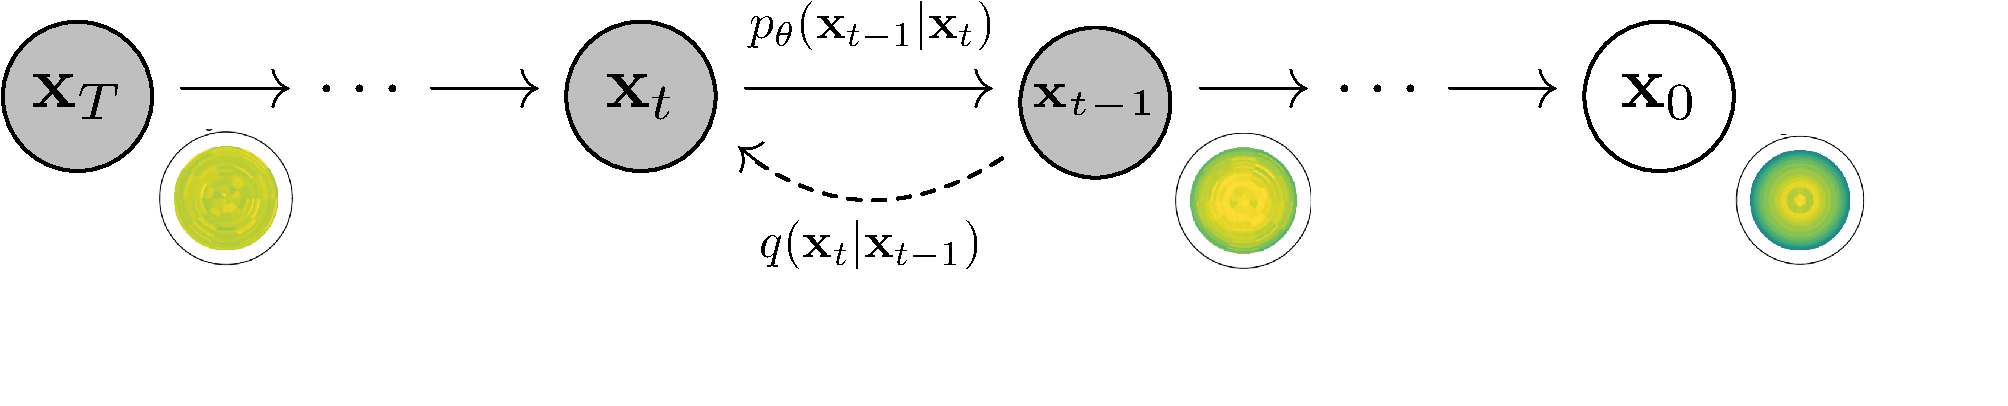
\includegraphics[width=0.95\myfigurewidth]{figures/pgm_diagram_xarrow_showers.pdf}
\caption{An illustration of the diffusion process, going from pure noise (left) to a realistic particle shower (right) in a transverse slice of a calorimeter. Adapted from Ref.~\cite{Ho:2020}.}
\label{fig:illus}
\end{figure}

The PI and his team developed the \diffu algorithm for the \challenge,
a recent community effort to compare different AI approaches to the simulation of particle showers in calorimeters, using common datasets and metrics.
The datasets include sampling calorimeters with varying materials and granularities and different particles including photons, pions, and electrons.
\diffu uses a convolutional U-net architecture~\cite{}, along with several innovations to handle the non-rectangular and sometimes irregular geometry of calorimeters.
The convolution operations are \textit{cylindrical}, accounting for periodicity in the azimuthal angle $\phi$.
The convolutions are \textit{conditional} on the longitudinal and radial coordinates, to account for violations of translation invariance in particle shower evolution.
Finally, a novel approach called Geometry Latent Mapping (\glam) is employed:
the model can learn two matrices that map between the calorimeter's irregular geometry and a regular grid suitable for convolutions.
Figure~\ref{fig:calodiffu} (left) shows results from the \challenge on the pion dataset, clearly demonstrating the superiority of \diffu,
which is found to produce the highest quality showers for all datasets~\cite{}.
The algorithms are compared based on metrics including classifier scores and the Fr\'echet particle distance~\cite{}.
This version of the algorithm is published in Ref.~\cite{};
subsequently, the quality has been improved even further, as shown in Fig.~\ref{calodiffu} (right), by adding a separate module that learns the per-layer deposited energy.

\begin{figure}[htb!]
\centering
\twofigeqh{figures/ds1-pions_CE_1.pdf}{figures/FCC_ERatio_dataset2_oct11_layer_norm_Diffu.pdf}
\caption{Left: example comparison of the separation power (for the shower center of energy) between \diffu, other algorithms, and \GEANTfour in the community \challenge.
Right: improved \diffu performance on the total deposited energy.}
\label{fig:calodiffu}
\end{figure}

The major remaining area for improvement in \diffu is its speed.
While it can still run 10--100 times faster than \GEANTfour by processing particles in large batches on GPUs,
the initial version required 400 denoising iterations or ``steps'' to produce high-quality output.
The improved version requires a factor of 4--8 fewer steps, depending on the dataset, because of its intrinsically higher quality.
More recently, some of the PI's colleagues have used \diffu as a platform to test further improvements to both the training and inference~\cite{},
and the most promising of these have been integrated into the model~\cite{}.
Numerous other avenues to make the algorithm faster while preserving quality are under investigation,
including latent diffusion~\cite{}, consistency models~\cite{}, and conditional distillation~\cite{}.
These illustrate a critical advantage of diffusion models:
because of the massive interest in these models in the broader ML community and in industry,
new methods are constantly being developed that can be easily imported for HEP use cases,
relying on the collaborative nature of open-source software.

Here, we propose to adapt \diffu to the more complex and variable CMS geometry.
The most involved case will be the High Granularity Calorimeter (HGCal), a part of the HL-LHC detector upgrades
that will increase the number of channels by almost two orders of magnitude.
The HGCal will have both hexagonal and rectangular cells in different regions, with different material types and thicknesses.
It is also the major driver of the predicted increase in \GEANTfour simulation time~\cite{}.
Further optimizations of the \diffu model will be needed to handle the high dimensionality and precision requirements of this new detector.
First, we will adapt the model to the existing, simpler CMS calorimeters,
which is both a useful stepping stone and an important ingredient for the dark QCD scan (Section~\ref{subsec:darkscan}).

\subsection{Refinement}\label{subsec:refine}

Conditional distillation is particularly interesting because it offers one path to enhance the existing CMS fast simulation chain (FastSim)~\cite{}.
Refining a low-quality simulation to obtain high-quality output was the objective of the PI's previous denoising project, which less used a less sophisticated AI architecture~\cite{}.
Diffusion models are much more capable, but so far the ``fully generative'' approach (producing a shower from pure noise) has been pursued;
this is because the sampling algorithms applied during the inference steps rely on the Gaussian nature of the noise.
The differences between FastSim and \GEANTfour will not be Gaussian, so while it should be easier to learn the difference between two similar distributions,
additional mathematical formalism must be derived in order to reuse the existing diffusion approach.
Instead, conditional distillation combines generation from pure noise with information from FastSim to modify the model to generate high-quality output in just one inference step.

The PI and his team have also developed a complementary high-level refinement, directly targeting analysis-level variables~\cite{}.
This algorithm includes the first use of the modified differential method of multipliers~\cite{} in HEP,
which automatically balances a tradeoff between ensemble and per-event comparisons when training the network.
With promising results on \cPqb-jet tagging variables, shown in Fig.~\ref{fig:refine},
the algorithm is now being expanded to cover other jet-related variables and validated for use in Run 3.
The approach can be understood as a significantly more precise, correlation-preserving alternative to traditional, manually-calculated correction factors.
Given that the CMS FastSim currently only agrees with \GEANTfour to within ${\sim}10\%$,
high-level refinement alone can substantially reduce the quality deficits in FastSim samples and the resulting uncertainties.

\begin{figure}[htb!]
\centering
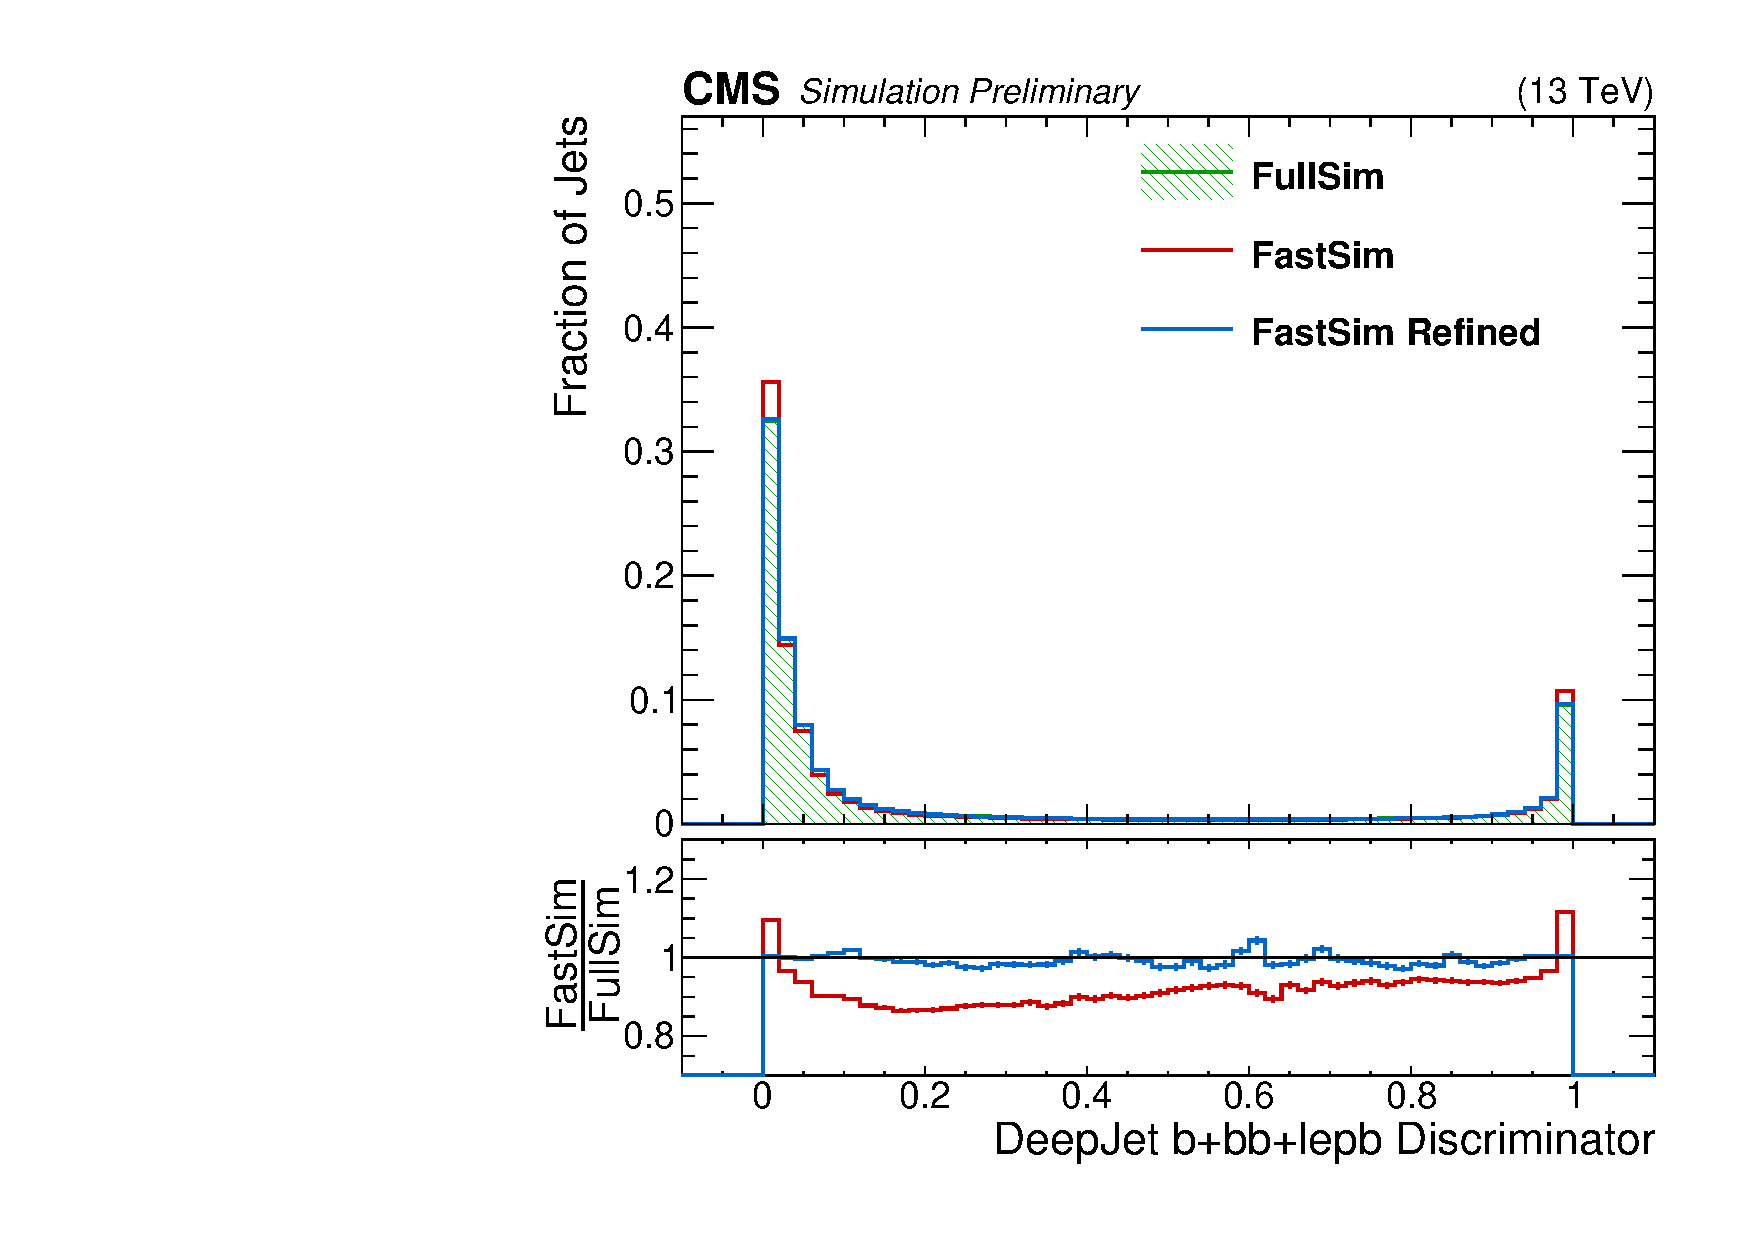
\includegraphics[width=0.5\myfigurewidth]{figures/Regression_20221127_DeepFlavB_preliminary}
\caption{The distribution of the \DEEPJET \cPqb-jet tagging discriminator, comparing \GEANTfour (FullSim), FastSim, and refined FastSim.}
\label{fig:refine}
\end{figure}

The combination of diffusion and refinement will be even more powerful.
In the chain FastSim~$\to$~diffusion~$\to$~refinement, each ML algorithm solves a progressively easier problem,
because the difference with respect to the previous step is smaller.
Therefore, it can learn the solution more precisely from a given dataset size, incorporating physics at different scales.
Essentially, refinement will address any residual disagreements between FastSim-based \diffu and \GEANTfour,
resulting in a more accurate final product, much like next-to-leading order matrix element calculations increase in accuracy by incorporating higher-order effects.

\subsection{Inference as a Service}\label{subsec:iaas}

\subsection{Future Colliders}\label{subsec:mucoll}
